We start by assuming a very simple generative model, relating the hidden neural activity (spike trains and intracellular calcium concnetrations) and the observations (fluorescence movies).  More specifically, we start by assuming we have collected a 1-dimensional fluorescence trace, $\bF=(F_1, \ldots, F_T)$ from a neuron.  At time $t$, the fluorescence measurement, $F_t$ is a linear-Gaussian function of the intracellular calcium concentration at that time, $C_t$:

\begin{align} \label{eq:F}
F_t &= \alpha (C_t + \beta) + \sig \varepsilon_t, \qquad \varepsilon_t \overset{iid}{\sim} \mN(0,1)
\end{align}

\noindent The scale, $\alpha$, absorbs all experimental variables impacting the scale of the signal, including number of sensors within the cell, photon$/\Del [$Ca$^{2+}]$ per sensor, amplification of imaging system, etc.  Similarly, the offset, $\beta$, absorbs baseline calcium concentration of the cell, background fluorescence of the fluorophore, imaging system offset, etc.  The standard deviation, $\sig$, results from calcium fluctuations independent of spiking activity, fluorescence fluctuations independent of calcium, and imaging noise. These three parameters therefore correspond to a number of simplifying assumptions, that we will relax in Section \ref{sec:results}.  

We further assume that the intracellular calcium concentration, $C_t$, jumps after each spike, and subsequently decays back down to rest with time constant, $\tau$, yielding $\tau (C_t-C_{t-1})/\Del = -C_{t-1} + n_t$.  Rearranging (and rescaling) a bit, we have:

\begin{align} \label{eq:C}
	C_t  &= \gam C_{t-1} + n_t, \qquad n_t \overset{iid}{\sim} \text{Poisson}(\lam \Del)
\end{align}

\noindent where $n_t$ indicates the number of times the neuron spiked at time $t$, and $\gam=1-\Del/\tau$. \footnote{This follows from writing \eqref{eq:C} as $\tau \frac{C_t - C_{t-1}}{\Del} = -C_{t-1} + n_t$.} Note that $C_t$ does not refer to absolute intracellular concentration of calcium but rather, a relative measure.  The assumed linearity of our model precludes the possibility of determining calcium in absolute terms (but see Section \ref{sec:nonlin} for a modified model).  Figure \ref{fig:schem} depicts a schematic illustration of this model. Note that the model, Eqs. \eqref{eq:F} and \eqref{eq:C} is a discrete-time state-space model.  Importantly, this model differs from the standard models in that we have a non-Gaussian noise term, $n_t$.  Thus, standard tools, such as the Kalman filter-smoother, cannot be applied directly.  We therefore develop a novel algorithm to handle problems of this nature, as described below.

\begin{figure}[H]
\centering 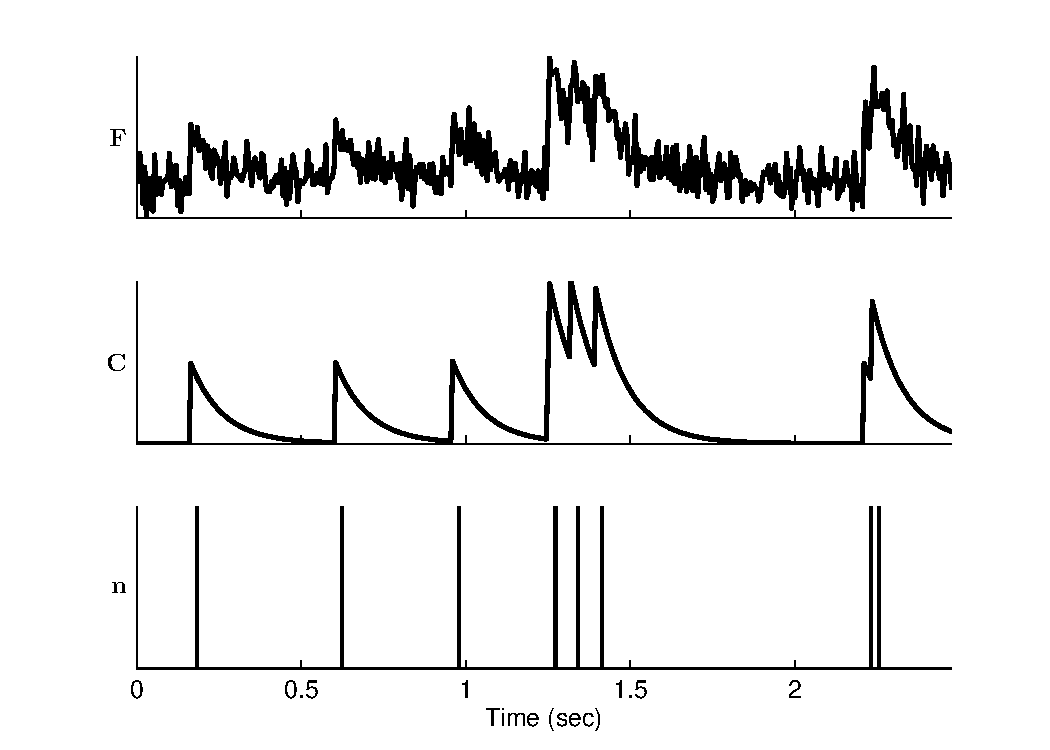
\includegraphics[width=.9\linewidth]{../figs/schem}
\caption{A schematic illustrating our model. The spike train (bottom panel) is convolved with an exponential with time constant $\tau$ to obtain the calcium dynamics (middle panel).  The fluorescence observations are simply the calcium dynamics, plus zero mean Gaussian noise (with variance $\sig^2$). Parameters: $\Del=5$ msec, $\alpha=1$ photons/$\mu$M, $\beta=0$ unitless, $\sig=0.25$ photons, $\tau=100$ msec, $\lam=5$ Hz.} \label{fig:schem}
\end{figure}


%relating spikes, $n_t$, baseline subtracted intracellular calcium concentration, denoted by $C_t$, and fluorescence measurements, $F_t$.  First, we assume a linear relationship between $F_t$ and $C_t$, with gaussian noise.  Second, we assume that $C_t$ jumps after each spike, and then decays according to some time constant.  Finally, we assume that spikes are distributed according to a Poisson process. The above assumptions lead to the follwoing model:

%. (1) spikes follow Poisson statistics with rate $\lam \Del$, (2) $C_t$ decays exponentially with decay $\gamma$ to baseline $\nu$, but jumps by $\rho$ after each spike, and (3) fluorescent observations are linear functions of $C_t$ with additive Gaussian noise with variance $\sig^2$.  Together, these assumptions imply the following model:

%\begin{align}
%\bF_t &= \balpha (C_t + \beta) +  \ve{\varepsilon}_t, \qquad &\ve{\varepsilon}_t \sim \mathcal{N}(\ve{0},\sig^2 \bI) \label{eq:obs} \\
%C_t  &= \gamma  C_{t-1} + n_t,  \qquad &n_t \sim \text{Poisson}(n_t; \lam \Del) \label{eq:trans}  
%\end{align}

%\noindent where $\balpha$ and $\beta$ set the fluorescence spatial filter and offset respectively, $\sig^2$ indicates the variance of the noise, and $\gamma$ sets the decay rate. 

%Note that   . To enforce identifiability, we will let $\balpha=1$ and $\beta=0$, without loss of generality, as explained below.


